\documentclass[a4paper,12pt]{article}
\usepackage[english]{babel}
\usepackage{setspace}
\usepackage[backend=bibtex, style=chicago-authordate]{biblatex}
\usepackage{graphicx} %for graphics
\usepackage{hyperref} %for links
\graphicspath{ {/home/heidi/Gradu2_0/Images/} }
\addbibresource{mastersthesis.bib}

\begin{document}
Structure of the work
	\begin{enumerate}
		\item Introduction \begin{itemize}
			\item Research questions
			\item Council of the Realm
			\item Sources \end{itemize}
		\item Method \begin{itemize}
			\item Defining the network
			\item Implementation of the network analysis
			\item Test run \end{itemize}
		\item Analysis
		\item Conclusion
	\end{enumerate}

Huomioita ja kysymyksiä 
\begin{itemize}
	\item Otsikko 0.1 on tekninen asia, korjaantuu itsestään
	\item Kappale Sources ja Test run ovat valmiimpaa tekstiä, välissä luonnosta
	\item Ovatko kuvaajat ja taulukot hyödyllisiä?
	\item Onko passiivi vai aktiivimuoto miellyttävämpää lukea?
	\item Ymmärtääkö tekstistä mitä teen ja miksi? 
\end{itemize}
\begin{onehalfspace}
\subsection{Sources}
Since this work is conducted with pre-collected dataset, this work can be categorized as secondary analysis. Secondary analysis meaning re-analyzing the data with new research questions or approaches, while primary analysis involves the collection of the data. Secondary analysis can also be discerned from meta analysis, which means comparing multiple previous studies (usually with quantitative methods) to create a synthesis on a certain question.\footcite[p. 4-5.]{meta-analysis} 

On the contrary in their articles Kimmo Elo and Olli Kleemola or Elo and Tiina Lintunen apply a network analysis on their own primary datasets.\footcites{eloAklee15}{LintunenAndElo2019} However, in the case of this work the benefit of doing secondary analysis is that the focus can be on the implementation and assessment of the method. Furthermore, the existing dataset will be automatically and manually re-examined for possible errors in the process, as will be discussed soon. 

As mentioned earlier, this work is based on the \textit{Swedish councillors of the Realm, 1523-1680} -dataset authored by Marko Hakanen and Ulla Koskinen. The dataset was published in 2017 and can be found in Digital repository of University of Jyväskylä under the license CC BY 4.0. The dataset was collected as a part of the research conducted for the anthology \textit{Personal Agency at the Swedish Age of Greatness 1560–1720}.

The dataset consists of information from 257 Swedish councillors of the realm. Each councillor has the following feature attributes: date of birth, year of death, year, date and age of appointment, noble rank, spouse(s) along with father's spouse and the individual's family links between other councillors. The councillors are identified with their full name and id number.\footcites[p. 48.]{HakanenAKoskinen2017}{councillorsDS}

\begin{table}[h]
	\centering
	\caption{Example rows of the dataset: Gyllenhorn, Joen Olsson and Natt och Dag, Måns Johansson (\cite{councillorsDS})} 
	\resizebox{\textwidth}{!}{%
		\begin{tabular}{|c | c | c | c | c | c | c | c | c | c|}
			\hline
			Name & No. & D.O.B. & † & Appointed & Date & Age & Noble rank & Family members in the council & Spouse(s) / Father of Spouse / Date of Marriage \\ 
			\hline
			Gyllenhorn, Joen Olsson & 82 & & 1556 & 1529 & 00.6. & & Uradel (Ancient Nobility) & Son-in-law 44 & Karin Bese/Nils Nilsson Bese/1529 \\
			\hline
			Natt och Dag, Måns Johansson & 142 & 1498 & 1555 & 1529 & 00.6. & 31 & Uradel (Ancient Nobility) & & Barbro Eriksdotter/Erik Turesson Bielke/ probably 27.6.1524 \\
			\hline
		\end{tabular}%
	}
\end{table}

Hakanen and Koskinen have compiled the data from secondary sources such as biographical registers and databases, biography collections, lineage databases and research literature. The dataset's sources are listed in the dataset and in the article written by Hakanen and Koskinen, those include for instance Nordic Family Book (Nordisk familjebok), National Biography of Finland (Finland's nationalbiografi, Kansallisbiografia), genealogies of old Swedish aristocratic families (Äldre svenska frälsesläkter) and further refereed literature.\footcites[p. 48, 76]{HakanenAKoskinen2017}{councillorsDS} As reported by Hakanen and Koskinen the dataset is collected using methodologies of collective biography, new prosopography and source criticism.\footcite[p. 48.]{HakanenAKoskinen2017}

Even though the dataset can be assessed as reliable and generally accurate, there is the general problem of some missing data. As seen in the example of Table 1, some of the councillors have missing attributes such as date of birth and therefore age of appointment. The missing attributes are most likely due the fact that during the time span of the dataset there was no standard of civil registration. 

The order of keeping parish registers (kyrkbok) was given in the Swedish Church Law 1686 (Kyrkio-Lag och Ordning), six years from the endpoint of the dataset. The Church Law made it mandatory for parish vicars to keep certain records and documents concerning the population and economy of the parish. Among other things these parish registers included the records of marriages, births, christens, deaths and funerals. Despite that the Swedish parish registers have been assessed exceptionally comprehensive by historians, there are some considerable deficiencies due to the differing circumstances and practices between parishes, furthermore some of the registers have been destroyed or lost. Even though some records do exist prior and post the Swedish Church Law 1686, they are notably dispersed.\footcite[p. 169-176.]{viikki94} A case in point: according to the Dictionary of Swedish National Biography (Svenskt biografiskt lexikon) the birth year of king Gustav Vasa (1495 or 1496) is also an estimate.\footcite{sbl_gustav_v} 

However, the focus of this work is not on the ages of the councillors but in their affiliations, so, the more relevant question is whether or not there are missing family links. 

(TODO write script and do some checking)

As the relatively large dataset is compiled by humans, it leaves some room for typos and errors. While producing the first experimental graph of the dataset, some empty data points were found. These "ghosts" were nodes with only id number and one or two links to the other councillors. All in all there were four "ghosts" with the id numbers 147 (linked to 18 and 152), 215 (linked to 217), 249 (linked to 269) and 254 (linked to 94). With the help of Marko Hakanen it was resolved that those "ghost" nodes were data points removed from the dataset as the authors found out they have not been official councillors, however, some references to their id numbers had been left to the dataset by accident. The "ghost" nodes will be removed from the latter graphs.

\section{Method}
%TODO computer aided network analysis <- distinction between 'verkostotutkimus' mentioned in Juuso Marttila's thesis. 
My method is computer aided (social) network analysis. It is one of the most implemented methods in the field of digital humanities. Generally network analysis has other more everyday applications, such as, the analysis of the internet as a network in the field of technology. Quite a few textbooks have been written on network analysis.

%Furthermore, in the field of technology network analysis does have some everyday application, such as the analysis of the internet. 

\subsection{Defining the network}
Network analysis combines mathematics, statistics and social sciences Primarily it is based on the mathematical graph theory. A graph is a representation of the network. Graph includes nodes (also called vertices) and edges (also called links and connections).

\begin{figure}[h]
	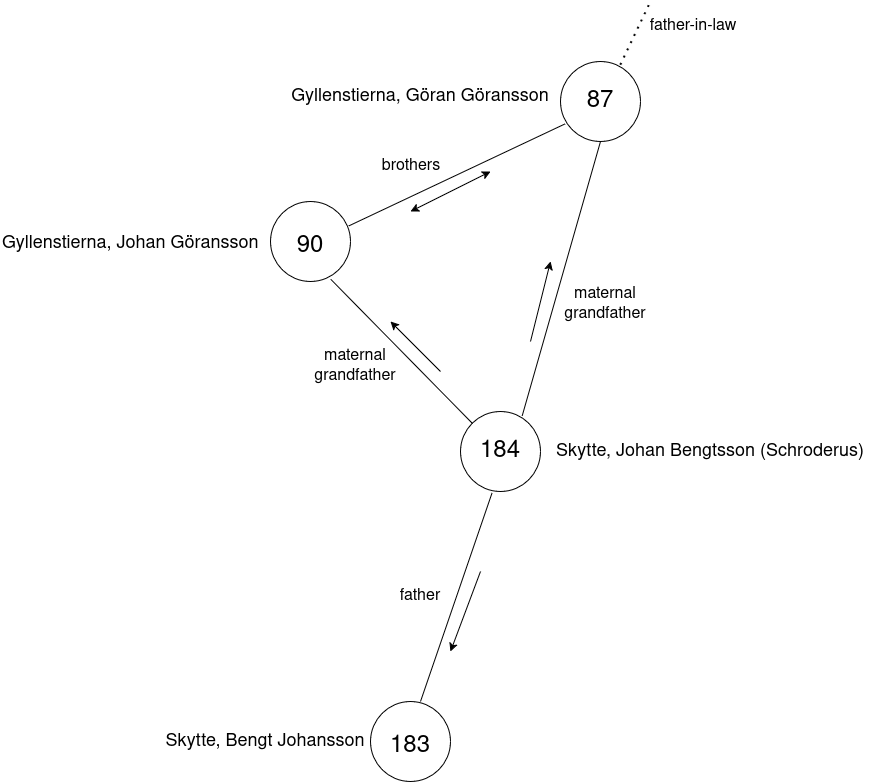
\includegraphics[scale=0.25]{example_network.drawio.png}
	\centering
	\caption{A sample from the graph} 
	\centering
\end{figure}
In this context the graph's nodes depict individual councillors with the input of name and id number. Correspondingly the edges represent the kinships between two nodes. For instance, in Figure 1 we can see that Johan Bengtsson (Schroderus) Skytte (id 184) is Bengt Johansson Skytte's (id 183) father and a maternal grandfather for Johan Göransson Gyllenstierna (id 90) and Göran Göransson Gyllenstierna (id 87). Johan Göransson and Göran Göransson are brothers, however, their father is not mentioned in the dataset. Göran Göransson also has further links in the network. \footfullcite{councillorsDS}

Calculating different statistics is a crucial part of the network analysis. One of the most important measures is the \textbf{node degree}. In all its simplicity node degree means the amount of edges connected to a specific node. For example, the degree of Johan Bengtsson (Schroderus) Skytte (id 184) is three or the degree of Bengt Johansson Skytte (id 183) is one. The \textbf{average degree} is the mean [keskiarvo] of all the node degrees of the specific graph. The \textbf{density} of the network is based on the node degrees. In very dense network almost every node is connected to each other, but a sparse graph has just a few edges in it.

Another important factor is whether the graph is \textbf{directed} or \textbf{undirected}. In directed graph the edges have directions, like in the communication networks a message has a sender and a receiver. The directions are marked with an arrow. In undirected graphs the edges are bidirectional (two way), for example, a relationship between two brothers can be understood as undirected. Directed graphs have more features and a more complex structures, for instance, the degrees of inbound and outbound edges can be counted separately. For simplicity, the graphs presented in this work are undirected.

\subsection{Implementation of the network analysis}
The data processing and analysis is conducted with a combination of Python programming language and Gephi software. Python is used for extracting the data from the councillors-dataset and formulating it in the right format: readable for Gephi. The actual network analysis, visualization and calculating statistics, is performed with Gephi. 

Python is a programming language popular amongst scientists. I selected Python due its simple syntax and ease in implementing small tasks like data processing. The language is understandable and widely used, which makes the work replicable. To be precise the script is written with Python 3.

As graphs are structures commonly used in programming, it would have been possible to conduct the actual network analysis using tools provided by Python, yet, Gephi software provides a visual user interface and more intuitive tools for the manipulation of the graph. Furthermore, the Gephi format makes the data and graph accessible also for non programmers.

Gephi is a software for network visualization and analysis. It contains tools for manipulating, filtering, clustering and visualizing the graph. It has built in appliances for fixing errors in data and calculating necessary statistics.\footcite{gephi} Gephi reads data from text format (comma separated values .csv) or Microsoft Excel tables (XLSX), and Gephi projects are saved as .gephi files. The processed graphs and data can be exported as images or tables.  

Nonetheless, Gephi does have some weaknesses. It is not always the most intuitive to use, and especially the visual configurations of the graph causes some issues. I have encountered difficulties with the node labels (the councilor's name next to the node). Sometimes the problems lies in the Gephi settings, but if the whole software crashes when trying to make the node labels visible, the problem lies within the software itself and should be solved when starting the program.\footnote{For Linux environments opening Gephi from command line with command "LIBGL\_ALWAYS\_SOFTWARE=1 ./gephi" can sometimes help.} 

Both of these tools are also open source and free to download. All scripts written for this work available on GitHub.\footnote{\url{https://github.com/Heidi-Suurkaulio/mastersthesis} TODO right link later}

Basically the steps of network analysis are : \begin{enumerate}
	\item Choosing the subject and data
	\item Pre processing the data for the network analysis
	\item Constructing the graph and finding possible issues and errors 
	\item Counting the statistics
	\item Deciding the layout (algorithm)
	\item Doing the interpretations
\end{enumerate}
However, the analysis is not that straightforward, sometimes the steps 2 and 3 must be repeated and re-repeated. Yet, on some circumstances the graph is not visualized or the statistics are not deemed important. These steps will be discussed in practice below.

\subsubsection{Test run}
%TODO add also to the source section about the end
%TODO fix councillor / councillor typo

To draft the structure of the graph and understand the nuances of the given data, a test run was carried out. The test run was done with a simple Python script, and no attention was paid to the temporal aspects of the network or the potential directions within the graph. The script and Gephi project used, and the visualization of the graph of the test run is available in GitHub in the TestRun folder\footnote{\url{https://github.com/Heidi-Suurkaulio/mastersthesis/tree/main/TestRun}}

The data processing was started by manually cleaning the data in LibreOffice Calc (equivalent to Microsoft Excel). The columns and rows containing information of the source material of the dataset and councillor's years active were removed. That made the structure of the data coherent and easier to manipulate with the Python script. The manually cleaned data is exported as .csv (comma separated values) file. The .csv file's header (the first line of the file) should be modified so that the column name "No." is changed to "Id" and "Family members in the council of the realm" is changed to "Family", the first one can cause an error if referenced in the Python code, the latter is inconveniently long. 

\begin{table}[h]
	\caption{Example of the raw .csv file}
	\resizebox{\textwidth}{!}{%
		\begin{tabular}{cccccccccp{1.5in}p{1.5in}}
			\hline
			1 &Name; &Id; &D.O.B.; &died; &Appointed; &Date; &Age; &Noble rank; &Family; &Spouse(s) / Father of Spouse / Date of Marriage \\
			\hline
			2 &Ingemar Petri; &162; &; &1530; &1495; &; &; &Estate unknown, Bishop; &; &; \\
			\hline
			3 &Tre Rosor, Ture Jönsson; &231; &; &1532; &1497; &; &; &Uradel (Ancient Nobility); &Father CR, Father-in-law CR, Sons 228, 230, Son (illegitimate) 175; &Anna Johansdotter/ Johan Christiernsson Vasa (CR) \\
			\hline
		\end{tabular}%
	}
\end{table}

The script itself reads the data from the .csv file. The connections between the councillors are separated from the "Family" column, based on the knowledge that each connection is marked with the id number of another councillor. The connections are then formatted and printed to .csv file. The connections .csv file containing values for "Source" id of the source concillor, "Target" id of target councillor, "Type" standard "Undirected", "Id" id number for the connection and "Weight" standard 1.0. Another .csv file is formatted and printed with the information of councillors' names and id numbers.

\begin{table}[h]
	\caption{Example of the connections .csv file}
	\centering
	\begin{tabular}{cccccc}
		\hline
		1 &Source, &Target, &Type, &Id, &Weight \\
		\hline
		2 &231, &228, &Undirected, &0, &1.0 \\
		\hline
		3 &231, &230, &Undirected, &1, &1.0 \\
		\hline
	\end{tabular}
\end{table}
\begin{table}[h]
	\caption{Example of the councillors .csv file}
	\centering
	\begin{tabular}{ccc}	
		\hline
		1 &Id; &Label \\
		\hline
		2 &162; &Ingemar Petri \\
		\hline
		3 &231; &Tre Rosor, Ture Jönsson \\
		\hline
	\end{tabular}
\end{table}

These .csv files are readable for Gephi. The outcome was an undirected graph of the councillors' affiliation network that had accumulated during the 160 years. The graph consisted of 261 nodes (257 real + 4 "ghosts") and 372 edges (including self loops and "ghost" nodes). The test run revealed three problems within the graph: the emergence of the empty "ghost" nodes, parallel edges and self loops. 

The "ghost" nodes were excess nodes with no name and only an id number and one or two connections in the graph. They were due to the references to the data points removed from the original dataset, and therefore can be ignored. The ghosts are discussed further in the subsection Sources. However, the more essential problem were parallel edges and self loops.

The parallel edges occur because one relationship, such as father and son, is sometimes marked doubly in the dataset. For example, in the case of Göran Göransson Gyllenstierna (id 87) the relatives are "Maternal Grandfather 184, Brother 90, Father-in-law 3, ...", and the same relationship is found in his grandfather's Johan Bengtsson (Schroderus) Skytte's (id 184) links: "Son 183, Grandson through daughter 87". Yet, the connection to Göran Göransson's brother Johan Göransson Gyllenstierna (id 90) is not marked in the grandfathers links. This means that the node of Göran Göransson Gyllenstierna (id 87) has one excess link compared to his brother's node. The case is visualized in the Figure 2.

\begin{figure}[h]
	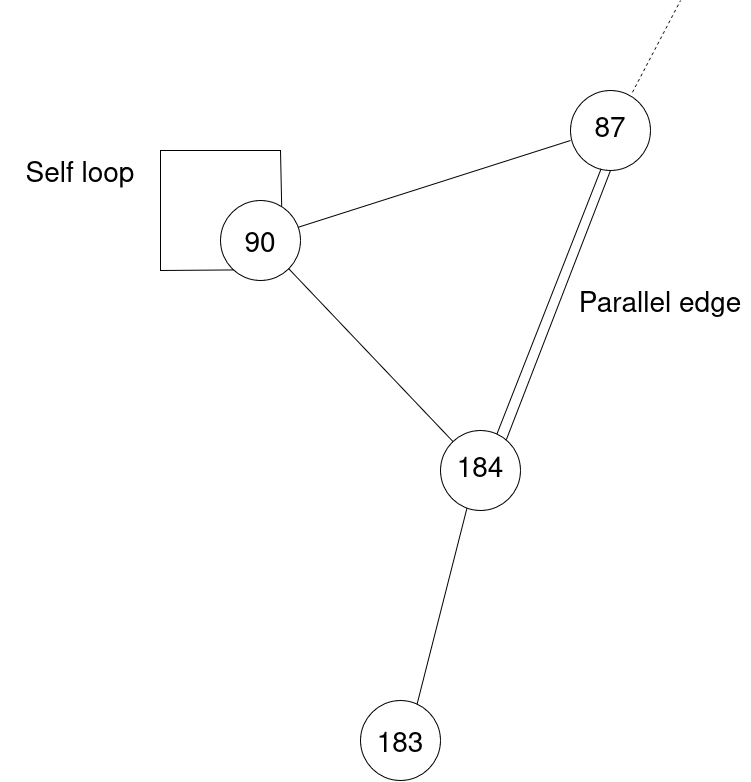
\includegraphics[scale=0.20]{double_link.drawio.png}
	\centering
	\caption{Visualisation of the parallel edge and self loop} 
	\centering
\end{figure}

These duplicate edges would cause bias to the calculation of the node degrees and any statistics based on them. A node degree is a sum of all the edges connected to one node, and if the relationships are inconsistently marked with one or two edges, the factually similar nodes would get different degrees. These inconsistent node degrees would accumulate when counting the average degrees an so forth. The problem of parallel edges is widely recognized in the field of network analysis, and therefore Gephi does have some builtin features for handling it.

While importing data to Gephi (on Import Spreadsheet) the strategy for merging the parallel edges can be chosen. One option is, for example, placing the sum or average of the parallel edges in the edge's degree, yet using only one connection to to represent the edge in the graph. In this context a more simple solution was chosen, with the option "First" Gephi will use only the first connection between two nodes ignoring any latter ones. This will reduce the amount of edges from 698 found in the connections.csv to only 372.

Self loops occur when one node has–for some reason or another–a connection to itself. Similarly to the parallel edges, they cause bias to the node degrees. In this graph a self loop can be found at least on the node with id 5 and id 90. In the case of id 5: Gustaf Axelsson Baner, his relatives are "Father 4, Father-in-law 217, Brother 9, Sons 5, 7, 8, 10, Sons-in-law 152 and 197", and similarly with id 90: Johan Göransson Gyllenstierna his family reads "Maternal Grandfather 184, Brother 90". These self loops are most likely caused by a typo in the dataset, because it is reasonable to assume that none is a son or brother to themselves.
 
Gephi does have a switch whether or not self loops are allowed in the graph, and it can automatically remove them based on the preference. The self loops are present in the test run graph alongside with the ghost nodes, yet those will be removed from the subsequent analysis. To highlight the ghosts they are colored cray, and the four nodes referred as an example here are colored red in the test run graph.

The last step in the preparation of the network analysis is the selection of the layout algorithm. For the test run an algorithm called Yifan Hu was used with default configurations except parameter theta set to 2.0. Then layout option "noOverlap" was chosen to separate possibly overlapping nodes, and some further manual placement of the nodes was done to make the graph more readable. The outcome was visually somewhat dense network in the middle and mostly unconnected isolated nodes around it. 

%TODO Problems: we don't have data about the women
\end{onehalfspace}
\printbibliography
\end{document}
